\documentclass[11pt]{report}
%\usepackage[margin=0.75in]{geometry}
\usepackage{geometry}
\usepackage[utf8]{inputenc}
\usepackage[greek, spanish, es-tabla]{babel}
\usepackage[bottom]{footmisc}
\usepackage[tt]{titlepic}
\usepackage{url}
\usepackage{xurl}
\usepackage{graphicx}
\usepackage{makeidx}
\usepackage{enumerate}
\usepackage{lastpage} % Para obtener la referencia a la última página
\usepackage{fancyhdr, ragged2e}
\usepackage{eurosym}
\usepackage{float}
\usepackage{titlesec}
\usepackage[bookmarks,hidelinks]{hyperref}
\usepackage{nameref}
\usepackage{enumitem}
\usepackage{booktabs}
\usepackage[table]{xcolor}
\usepackage{multirow}
\usepackage{amsmath}

\usepackage{listings}

	\addtolength{\oddsidemargin}{-.8in}
	\addtolength{\evensidemargin}{-.8in}
	\addtolength{\textwidth}{1.45in}

	\addtolength{\topmargin}{-.1in}
	\addtolength{\textheight}{1.25in}

\graphicspath{{figures/}}
\pagestyle{fancy}
\renewcommand{\chaptermark}[1]{\markboth{\scriptsize\MakeUppercase{#1}}{}}
\renewcommand{\sectionmark}[1]{\markright{\tiny\MakeUppercase{#1}}{}}

\fancypagestyle{plain}{
    \fancyhf{}
    \renewcommand{\headrulewidth}{0pt} 
    \fancyfoot[L]{\raisebox{-0.6cm}{
\includegraphics[height=1cm]{figures/EscudoUniovi.jpg}}}
    \fancyfoot[C]{\scriptsize BidMon Universe. Plataforma de coleccionismo de cartas digitales. \\ Trabajo Fin de Grado Ingeniería Informática del Software \textbar{} Versión 0.1 \\ Paula Suárez Prieto}
    \fancyfoot[R]{\thepage\ de \pageref{LastPage}}
    \renewcommand{\footrulewidth}{0.4pt}
}

%Evita warnings de cabecera
\setlength{\headheight}{15pt}
\setcounter{secnumdepth}{4}

%Esto es para poder ponerle un formato bien hecho a los \paragraph{}
\titleformat{\paragraph}
{\normalfont\normalsize\bfseries}{\theparagraph}{1em}{}
\titlespacing*{\paragraph}
{0pt}{3.25ex plus 1ex minus .2ex}{1.5ex plus .2ex}

%Y esto para para ponerselo a los \subparagraph{}
\titleformat{\subparagraph}
{\normalfont\normalsize\bfseries}{\theparagraph}{1em}{}
\titlespacing*{\subparagraph}
{0pt}{1ex plus 1ex minus .2ex}{1.5ex plus .2ex}

% Configuración para permitir la numeración hasta el quinto nivel
\setcounter{secnumdepth}{5}

% Crear un nuevo contador para subsubsubsection que se reinicia con cada subsubsection
\newcounter{subsubsubsection}[subsubsection]

% Formatear el contador para que se muestre como subsubsection.subsubsubsection
\renewcommand{\thesubsubsubsection}{\thesubsubsection.\arabic{subsubsubsection}}

% Definir el comando subsubsubsection
\newcommand{\subsubsubsection}[1]{%
  \refstepcounter{subsubsubsection}
  \paragraph{#1}\mbox{}\\
}

% Formato para el título de subsubsubsection
\titleformat{\paragraph}
  {\normalfont\normalsize\bfseries\itshape}{\thesubsubsubsection}{1em}{}
\titlespacing*{\paragraph}
  {0pt}{3.25ex plus 1ex minus .2ex}{-1ex plus .2ex}

  
\makeindex

\begin{document}
\selectlanguage{spanish} 

\hypersetup{pageanchor=false}
\begin{titlepage}
	\centering
	
\includegraphics[width=0.2\textwidth]{EscudoUniovi}
	\hspace{3 cm}
	
\includegraphics[width=0.3\textwidth]{EscudoEscuela}
	\par\vspace{1cm}
	
	\vspace{1.5cm}
	{\huge\bfseries BidMon Universe \\ Plataforma de coleccionismo de cartas digitales\par}
	\vspace{2cm}
	{\large \textbf{GRADO EN INGENIERÍA INFORMÁTICA DEL SOFTWARE} \par}
	\vspace{1cm}
	{\scshape\Large Trabajo Fin de Grado\par}
	%\vfill
   	
  \vspace{2cm}
	%\vfill
	\textbf{AUTOR}\par
	Paula Suárez Prieto \\
	%\vfill
	\vspace{1.5cm}
	%{\Large\itshape ((Nombre del Alumno))\par}
	%\vfill
	\textbf{TUTOR}\par
	Hugo Lebredo Buján
	\vfill
	
	{\large Julio 2024 \par}
\end{titlepage}


\newpage
\pagestyle{plain}
Copyright (C) 2020 \textbf{ELENA ALLEGUE GONZÁLEZ, JOSÉ MANUEL REDONDO LÓPEZ} \\
Teaching Innovation Project: PINN-19-A-029 (University of Oviedo)\\
This work has been published in \cite{RedondoPlantillasRG19} \cite{RedondoUCO20}\\
\\
Esta versión de la plantilla para Trabajos de Fin de Grado ha sido posible gracias a la donación de la ex-alumna Elena Allegue González de su documentación de Trabajo de Fin de Grado, que ha servido como base para elaborar esta versión. Aquí podréis encontrar todos los títulos y subtítulos de las secciones, pero las explicaciones se mantendrán en la versión \textit{Word} de la plantilla (se proporciona una versión PDF de la misma para facilitar el acceso a las mismas). No obstante, del trabajo de Elena se han conservado ejemplos de como hacer elementos clave como imágenes, tablas, etc.

Desarrollar una versión \textit{Latex} de la plantilla desde cero es una trabajo bastante largo, pero gracias al trabajo de Elena se ha podido equiparar esta versión con las de \textit{Word} mucho más rápidamente.

%\newpage
\pagestyle{fancy}
\chapter*{Agradecimientos}

\pagestyle{fancy}

\renewcommand{\chaptermark}[1]{\markboth{\scriptsize\MakeUppercase{#1}}{}}
\renewcommand{\sectionmark}[1]{\markright{\tiny\MakeUppercase{#1}}{}}



%\Configuración del pie de página

\fancyfoot{}
\fancyfoot[L]{\raisebox{-0.6cm}{
\includegraphics[height=1cm]{figures/EscudoUniovi.jpg}}}

\fancyfoot[R] {\thepage\ de \pageref{LastPage}}
\fancyfoot[C]{\scriptsize BidMon Universe. Plataforma de coleccionismo de cartas digitales. \\ Trabajo Fin de Grado Ingeniería Informática del Software \textbar{} Versión 0.1 \\ Paula Suárez Prieto   }
\setlength{\footskip}{32.93277pt}
\renewcommand{\footrulewidth}{0.4pt}
\pagenumbering{arabic}

%\newpage


\pagestyle{plain}


\setcounter{tocdepth}{2}
\setcounter{secnumdepth}{4}
\pagestyle{plain}
{
  \renewcommand{\thispagestyle}[1]{}
  \tableofcontents
}
\clearpage


\newpage
{
  \renewcommand{\thispagestyle}[1]{}
  \listoffigures
}
\clearpage

\newpage
{
  \renewcommand{\thispagestyle}[1]{}
  \listoftables
}
\clearpage

\newpage
\hypersetup{pageanchor=true}

\newpage


\newpage
\thispagestyle{empty}
\chapter{Introducción}
\section{Resumen}


\section{Palabras Clave}


\section{Abstract}


\section{Keywords}

\pagestyle{fancy}
%\newpage
\chapter{PLANIFICACIÓN DEL SISTEMA DE INFORMACIÓN}


\newpage

\section{INICIO DEL PLAN DE SISTEMAS DE INFORMACIÓN}
 
\subsection{Identificación del Alcance del Plan de Sistemas de Información }


\subsection{Determinación de Responsables}


\newpage
\section{DEFINICIÓN Y ORGANIZACIÓN DEL PLAN DE SISTEMAS DE INFORMACIÓN}
 

\subsection{Especificación del Ámbito y Alcance} 


\subsection{Organización del Plan de Sistemas de Información }



\newpage
\section{ESTUDIO DE LA INFORMACIÓN RELEVANTE}
 
\subsection{Selección y Análisis de Antecedentes} 


%\newpage
\chapter{DEFINICIÓN DE LA ARQUITECTURA TECNOLÓGICA}

\newpage

\section{Identificación de las Necesidades de Infraestructura Tecnológica} 

\newpage
\section{Selección de la Arquitectura Tecnológica} 

\newpage
\chapter{ESTUDIO DE VIABILIDAD DEL SISTEMA}
	
\newpage


\section{ESTUDIO Y VALORACIÓN DE ALTERNATIVAS DE SOLUCIÓN. SELECCIÓN DE ALTERNATIVA FINAL}

\section{Análisis de sistemas similares}

En este apartado, se aborda un análisis detallado de las plataformas y sistemas que actualmente exhiben un comportamiento similar al del sistema que se pretende desarrollar para 'BidMon Universe'. 

La realización de este análisis es muy importante, ya que proporciona una base sólida para la toma de decisiones estratégicas. Al examinar detenidamente tanto las ventajas como las desventajas de los sistemas existentes, se identifican estrategias exitosas y se reconocen posibles fallos 
o áreas susceptibles de mejora. Este enfoque no solo informa las decisiones de diseño y tecnología, sino que también las fundamenta en un conocimiento práctico y bien contextualizado. Así, se garantiza que el desarrollo de 'BidMon Universe' esté 
armonizado con las tendencias actuales y adopte las soluciones más efectivas y adecuadas para su propósito.

El objetivo del proyecto es permitir a los usuarios coleccionar cartas e intercambiarlas mediante subastas, específicamente cartas de Pokémon. Por esta razón, se ha llevado a cabo un análisis de sistemas similares enfocados en los siguientes puntos:
\begin{itemize}
    \item Sistemas de intercambio de cartas digitales: Se analizarán diversos sistemas de intercambio de cartas digitales, destacando su relevancia en el mercado y las funcionalidades que ofrecen.
    \item Sistemas de subastas en línea: Se evaluarán plataformas de subastas en línea, analizando sus ventajas y desventajas, con el objetivo de identificar las mejores prácticas aplicables a nuestro proyecto.
    \item El mercado de coleccionistas de Pokémon: Se estudiará la extensa base de seguidores y coleccionistas de cartas Pokémon, comprendiendo su comportamiento, preferencias y el impacto que tienen en el mercado de subastas.
\end{itemize}

\subsection{Análisis de sistemas de intercambio de cartas digitales}
En esta sección se analizarán los sistemas de intercambio de cartas digitales, como EA Sports FC, NBA 2K y LaLiga Fantasy, que permiten a los usuarios adquirir y vender cartas de jugadores. 
Aunque el sistema de coleccionismo de cartas puede variar según la plataforma del juego, todos comparten una serie de características comunes. Estas incluyen la posibilidad de pujar 
por un jugador o comprarlo directamente, la existencia de distintas rarezas de cartas y la inclusión de eventos especiales.

\subsubsection{EA Sports FC}
\coloredUnderline{\href{https://www.ea.com/es-es/games/ea-sports-fc}{EA Sports FC}} es una destacada franquicia de videojuegos de fútbol disponible en diversas plataformas. 
Este análisis se centrará en el modo de juego \coloredUnderline{\href{https://www.ea.com/es-es/games/fifa/fifa-23/ultimate-team/item-guide}{FIFA Ultimate Team}}, 
que busca transformar la interacción de los jugadores, permitiéndoles construir y gestionar su propio equipo de fútbol. Los usuarios pueden buscar jugadores en el mercado de transferibles, 
pujar por ellos o comprarlos directamente. Además, pueden incrementar el valor de sus jugadores completando desafíos y cambiar la apariencia de las cartas. 
Este modo incluye tarjetas de jugadores con distintas rarezas, haciendo que algunas sean más valiosas que otras.

Se estima que EA Sports FC ha generado más de 6.000 millones de dólares en ingresos netos entre 2020 y 2025\cite{sanmartin000MillonesDolares2021}. En 2020, 
los ingresos casi se triplicaron en comparación con 2015, demostrando un crecimiento exponencial. El informe anual de Electronic Arts para el año fiscal 2023\cite{ea2023} 
especifica que se generaron 7.426 millones de dólares en ingresos netos y revela que el modo Ultimate Team de FIFA 23 es el más popular de la franquicia, con más de 10 millones 
de jugadores activos mensuales, siendo una de las mayores fuentes de ingresos de la empresa. El informe también destaca la intención de continuar desarrollando este mercado 
mediante la incorporación de nuevas características para el modo Ultimate Team.

La popularidad de este modo de juego ha llevado a Electronic Arts a lanzar una aplicación móvil llamada \coloredUnderline{\href{https://apps.apple.com/es/app/ea-sports-fc-24-companion/id1127108818}{EA SPORTS FC™ 24 Companion}}, 
que permite a los usuarios gestionar su club de FIFA Ultimate Team desde dispositivos móviles. Los usuarios necesitan tener el juego FIFA 24 para utilizar la aplicación, 
la cual se conecta a la cuenta del usuario en el juego. 

Desde la aplicación, los usuarios pueden comprar sobres de cartas, gestionar su plantilla, comprar jugadores en el mercado de transferibles y pujar por jugadores en subastas para utilizarlos posteriormente en el juego. 
Esta aplicación permite a los usuarios estar al tanto de las últimas novedades y ofertas del mercado, así como recibir notificaciones en tiempo real sobre el estado de sus pujas.

En las siguientes figuras, se muestra la interfaz de usuario de EA SPORTS FC™ 24 Companion.

\begin{figure}[H]
    \centering
    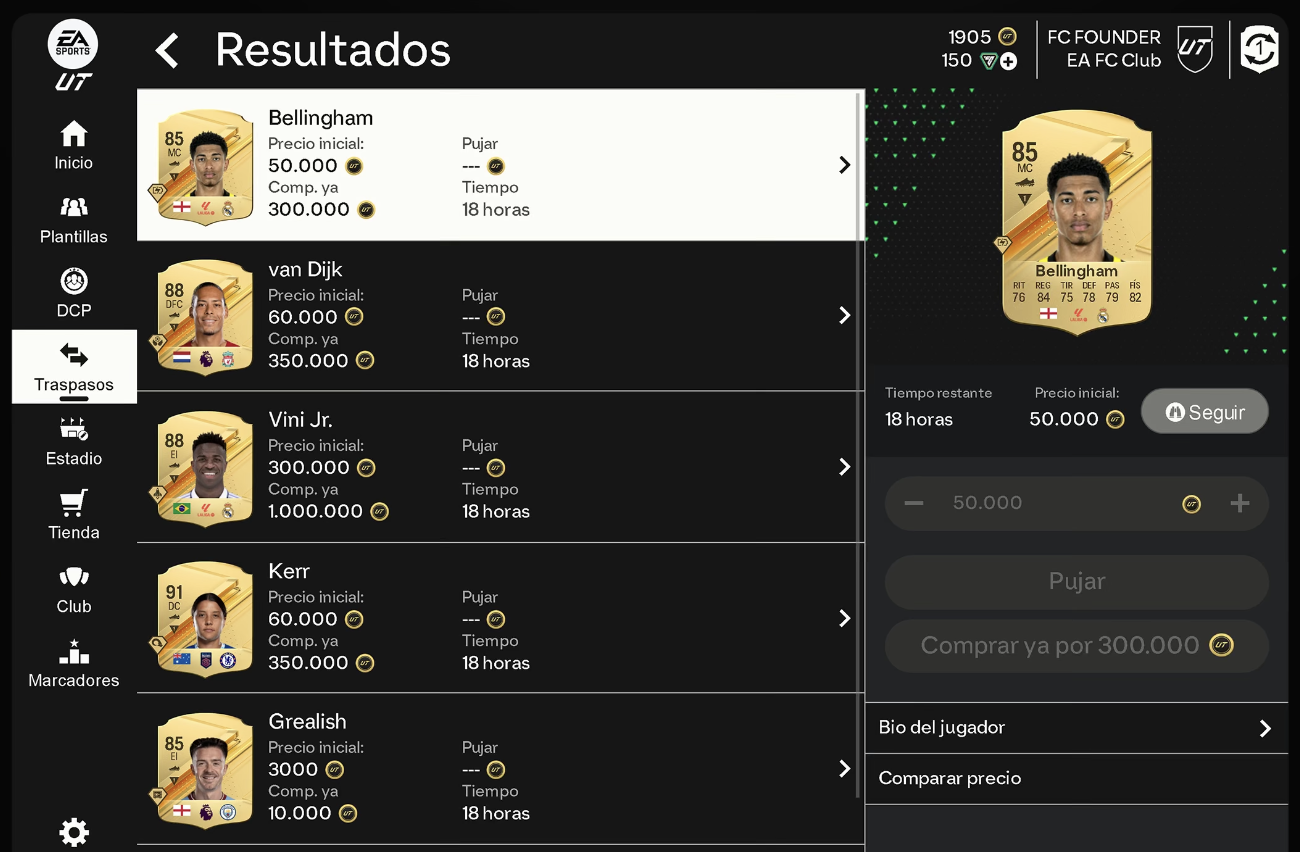
\includegraphics[width=0.7\textwidth]{figures/4-Estudio-viabilidad/4_FC_Companion.png}
    \caption{Página de traspasos de jugadores de EA SPORTS FC™ 24 Companion}
    \label{fig:ea_sports_fc_1}
    \hypertarget{fig:ea_sports_fc_1}{}
\end{figure}

\begin{figure}[H]
    \centering
    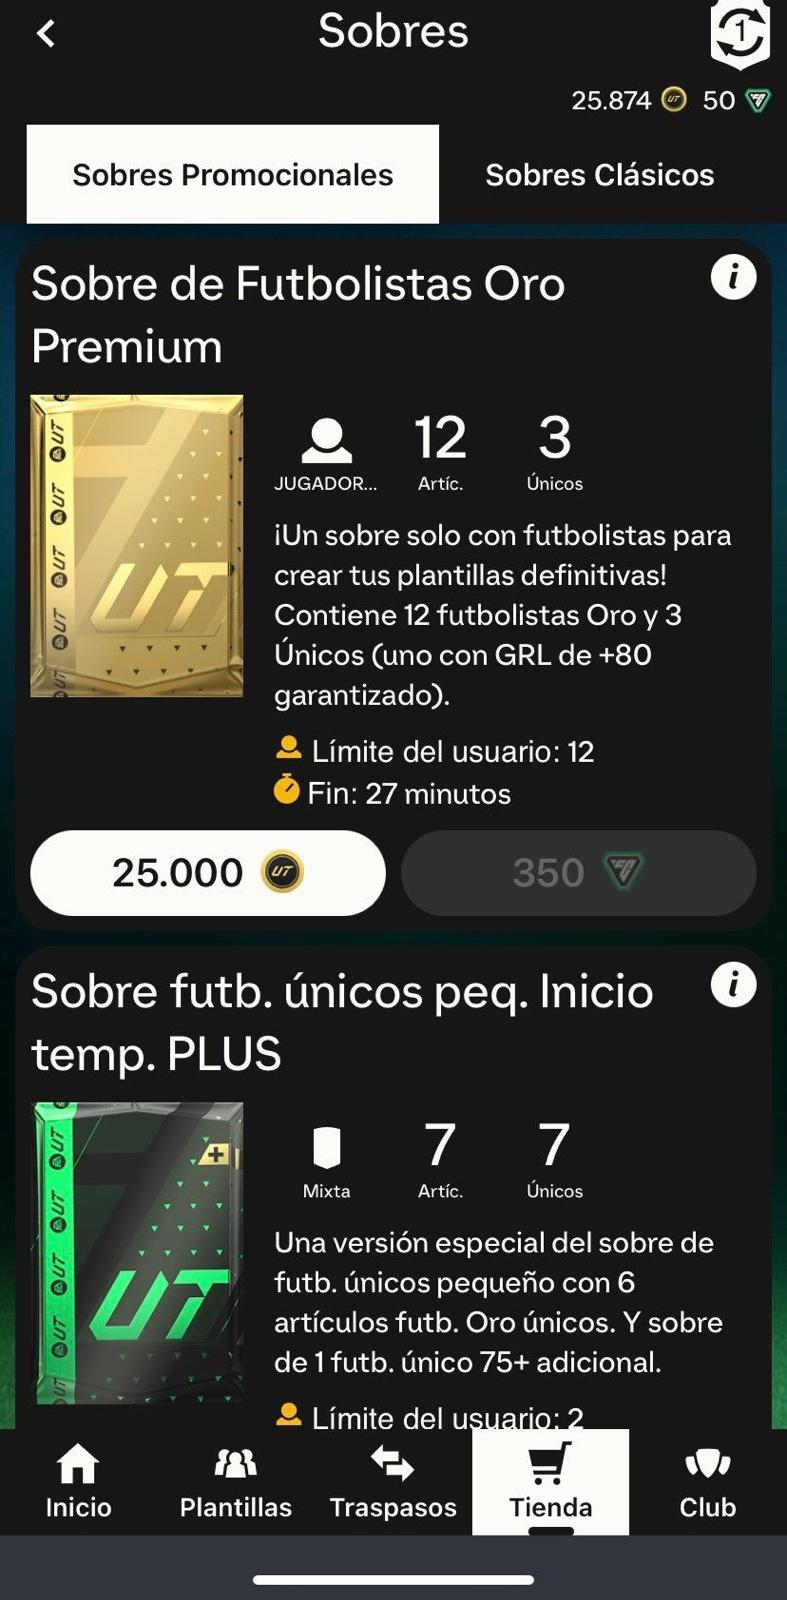
\includegraphics[width=0.3\textwidth]{figures/4-Estudio-viabilidad/4_FC_Companion2.jpeg}
    \caption{Página de compra de sobres de EA SPORTS FC™ 24 Companion}
    \label{fig:ea_sports_fc_2}
    \hypertarget{fig:ea_sports_fc_2}{}
\end{figure}

\subsubsubsection{Ventajas de EA Sports FC}
En el contexto de EA Sports FC, destacan las siguientes ventajas:
\begin{itemize}
    \item Los usuarios pueden marcar una carta para efectuar un seguimiento y recibir notificaciones en caso de una disminución en su precio.
    \item Se proporcionan estadísticas detalladas de cada carta, incluyendo su evolución de precio en las últimas semanas, así como los valores más bajos y más altos a los que se está vendiendo actualmente.
    \item Existe la opción de vender una carta directamente, evitando la necesidad de utilizar el sistema de subastas. 
    \item Cuenta con un buscador de ofertas que incorpora varios filtros.
    \item Los usuarios tienen la posibilidad de editar o cancelar sus pujas en curso.
    \item El sistema de subastas implementado opera bajo un mecanismo de puja ciega.
\end{itemize}

\subsubsubsection{Desventajas de EA Sports FC}
Sin embargo, es importante mencionar algunas desventajas de EA Sports FC, que incluyen:
\begin{itemize}
    \item Un número limitado de órdenes de canje simultáneas como, por ejemplo, el máximo de 25 permitido en EA Sports FC Mobile.
    \item Las pujas solo se pueden realizar por un valor igual o superior al establecido por el juego. 
\end{itemize}

\subsubsubsection{Ventajas del nuevo sistema respecto EA Sports FC}
El sistema en desarrollo presenta varias características que mejoran la experiencia del usuario en comparación con EA Sports FC.

\begin{itemize}
    \item El acceso a la aplicación es completamente gratuito.
    \item Ofrece una mayor personalización en el proceso de puja, brindando a los usuarios una experiencia más flexible y adaptada a sus preferencias.
    \item El usuario tiene la posibilidad de acceder a un histórico exhaustivo en el que se detallan todas las transacciones realizadas.
\end{itemize}

\subsubsection{NBA 2K}
\coloredUnderline{\href{https://nba.2k.com/}{NBA 2K}} es una destacada franquicia de videojuegos de baloncesto disponible en diversas plataformas. 
Este análisis se centrará en el modo de juego \coloredUnderline{\href{https://nba.2k.com/2k24/es-ES/myteam/}{MyTEAM}}, 
que busca transformar la interacción de los jugadores, permitiéndoles construir y gestionar su propio equipo de baloncesto. Los usuarios pueden buscar jugadores en el mercado de transferibles, 
pujar por ellos o comprarlos directamente. Existen distintos niveles de cartas para añadir un elemento de emoción al juego.
Existen también cartas de recompensa que se pueden obtener completando desafíos y eventos especiales.

Se estima que NBA 2K ha generado ingresos significativos en los últimos años. En el año fiscal 2023, 
los ingresos de Take-Two Interactive alcanzaron niveles récord gracias a sus franquicias principales, incluyendo NBA 2K. El informe anual de Take-Two Interactive para el año fiscal 2023\cite{take_two_2023} 
destaca que NBA 2K es una de las mayores fuentes de ingresos de la empresa, con una base de usuarios activa y comprometida, especialmente en el modo MyTEAM. 
En el informe se menciona la intención de seguir desarrollando este mercado ya que se espera que continúe creciendo en los próximos años.

La popularidad de este modo de juego ha llevado a Take-Two Interactive a lanzar una aplicación móvil llamada \coloredUnderline{\href{https://nba.2k.com/2k24/mynba-2k24/}{MyNBA 2K Companion App}}, 
que permite a los usuarios gestionar su equipo de MyTEAM desde dispositivos móviles. Los usuarios necesitan tener una cuenta de NBA 2K para utilizar la aplicación, 
la cual se conecta a la cuenta del usuario en el juego. 

La aplicaicón permite a los usuarios comprar sobres de cartas, gestionar su plantilla, comprar jugadores en el mercado de transferibles y pujar por jugadores en subastas para utilizarlos posteriormente en el juego.
Tiene otras funciones interesantes como la posibilidad de personalizar su propio jugador por medio de la función de escaneo facial, la cual permite a los usuarios escanear su rostro y añadirlo al juego.

En las siguientes figuras, se muestra la interfaz de usuario de NBA 2K Mobile.


\subsubsection{LaLiga Fantasy}
\coloredUnderline{\href{https://laligafantasy.relevo.com/}{LaLiga Fantasy}} un juego basado en la liga de fútbol española, conocida como LaLiga. En este juego, los usuarios tienen la capacidad de crear equipos que se componen de jugadores cuyo rendimiento se correlaciona con el desempeño real en los partidos de LaLiga. Además, existe la posibilidad de competir por premios reales en determinadas instancias del juego.
El juego dispone de un mercado en el que los usuarios pueden vender o adquirir jugadores a través de un sistema de subastas, por lo que estamos ante un escenario similar al anterior.

A continuación, se muestra la interfaz de usuario de LaLiga Fantasy.
\begin{figure}[H]
    \centering
    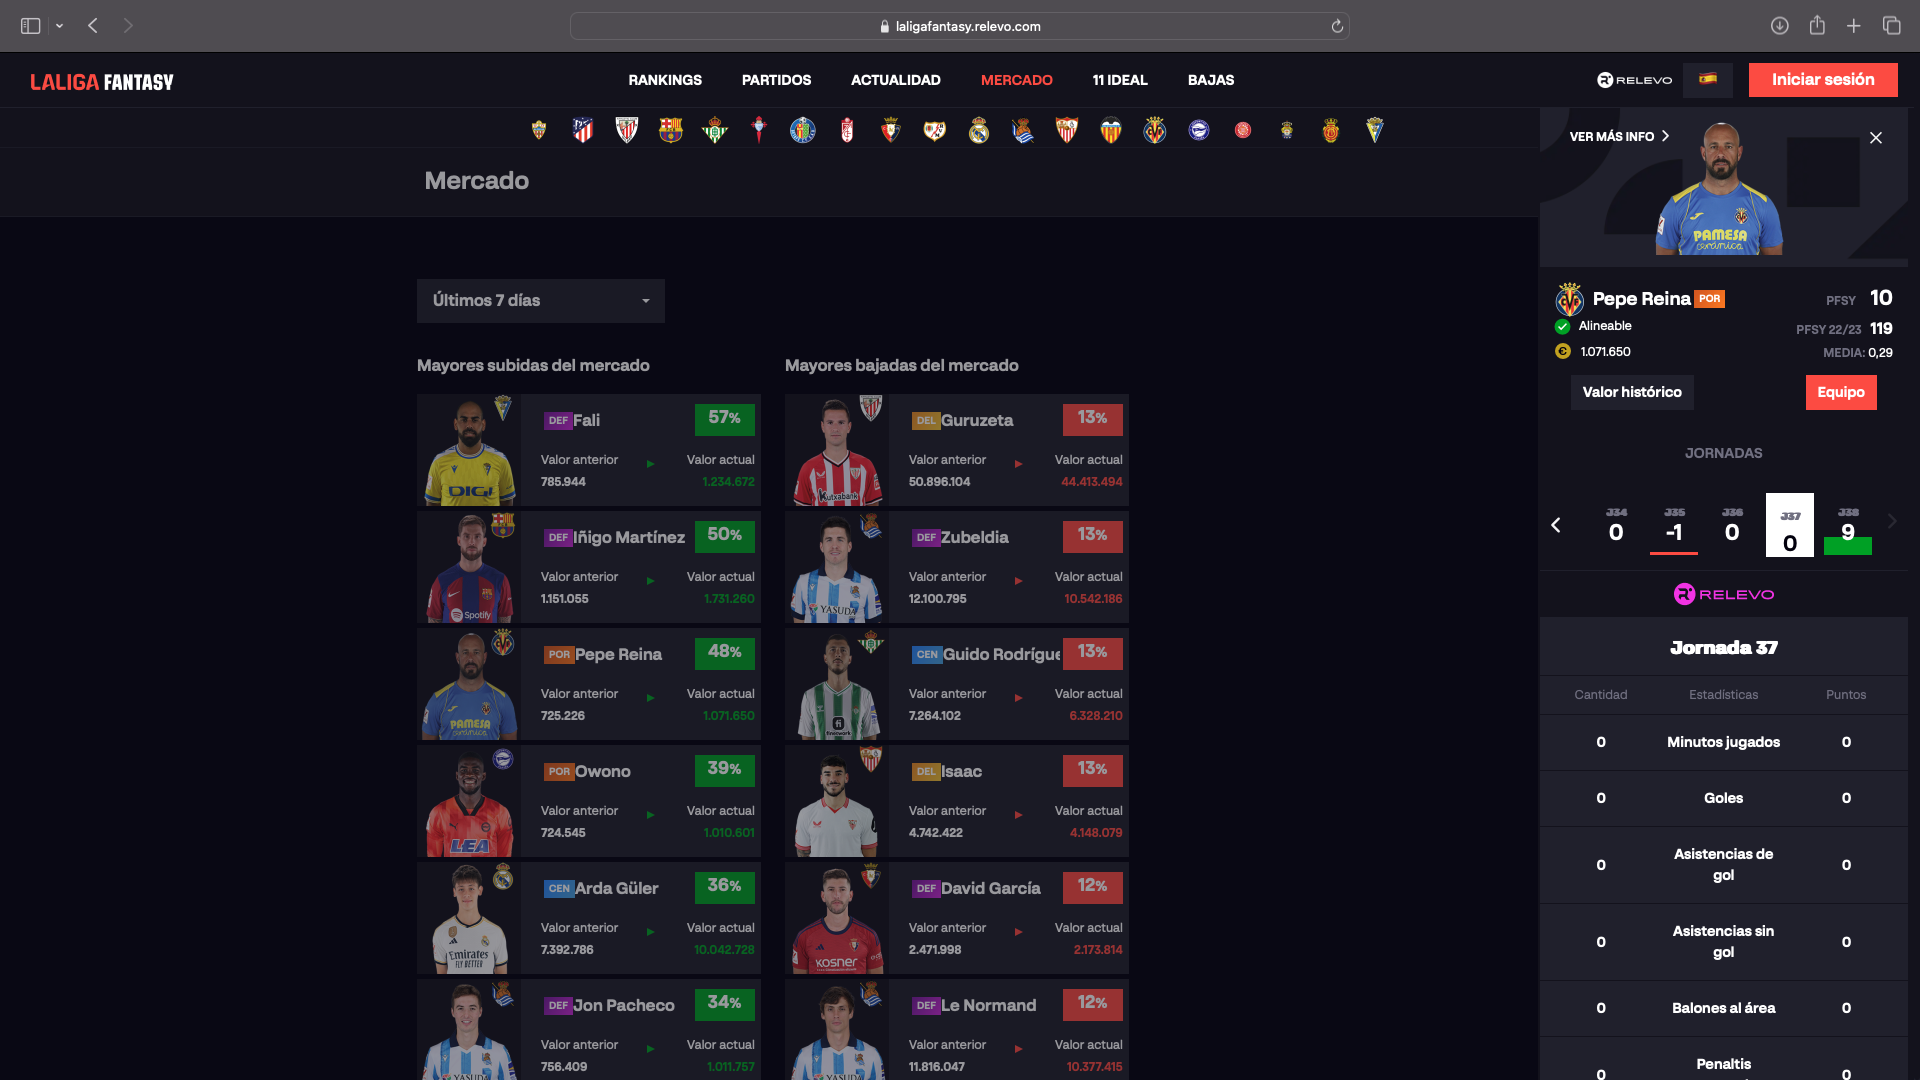
\includegraphics[width=0.7\textwidth]{figures/4-Estudio-viabilidad/4_LaLigaFantasy.png}
    \caption{Página de mercado de jugadores de LaLiga Fantasy}
    \label{fig:la_liga_fantasy}
    \hypertarget{fig:la_liga_fantasy}{}
\end{figure}

\subsubsubsection{Ventajas de LaLiga Fantasy}
Dentro del marco de LaLiga Fantasy, se destacan las siguientes características:
\begin{itemize}
    \item El juego renueva constantemente el mercado de transferibles.
    \item El juego cuenta con la capacidad de generar ofertas automáticas por los futbolistas que se encuentran en venta. Estas ofertas se establecen a partir de un valor aleatorio que oscila entre el valor de mercado del jugador, con un margen del 10\% tanto por encima como por debajo de dicho valor.
    \item Recientemente se ha incorporado el mercado de ``clausulazos'', donde los usuarios pueden adquirir un jugador pagando su cláusula, que será más elevada que el valor de mercado, sin tener que depender del propietario del jugador.
    \item Se pueden realizar ofertas por jugadores a otros usuarios.
\end{itemize}

\subsubsubsection{Desventajas de LaLiga Fantasy}
Se pueden identificar las siguientes desventajas:
\begin{itemize}
    \item La limitación a un máximo de 24 jugadores en la plantilla, lo que puede ocasionar la pérdida de oportunidades en subastas.
    \item La plataforma brinda escasa flexibilidad en lo que respecta a la personalización al momento de poner un jugador en venta.
\end{itemize}

\subsubsubsection{Ventajas del nuevo sistema respecto LaLiga Fantasy}
\begin{itemize}
    \item LaLiga Fantasy ofrece una suscripción de 0,99€/mes para poder jugar sin anuncios mientras que el sistema que se desarrollará carece de anuncios.
    \item Se proporciona un historial de transacciones completo para que los usuarios puedan rastrear las compras y ventas.
    \item Se implementa un sistema de subastas en tiempo real que, además, brinda una mayor personalización al usuario en aspectos como la duración de la subasta y los valores de venta, entre otros.
    \item Además de acceder al mercado, los usuarios tienen la opción de adquirir sobres de cartas, lo que añade un elemento de emoción a la aplicación.
\end{itemize}

\subsubsection{eBay}
\coloredUnderline{\href{https://www.ebay.es/}{eBay}} es una plataforma de comercio online que permite a los usuarios comprar y vender productos a través de subastas o ventas directas. Se puede encontrar una sección específica dedicada al coleccionismo, donde los usuarios pueden pujar por artículos de interés, como cartas.

En la siguiente figura, se muestra la interfaz de usuario de la sección de coleccionismo de cartas de eBay.
\begin{figure}[H]
    \centering
    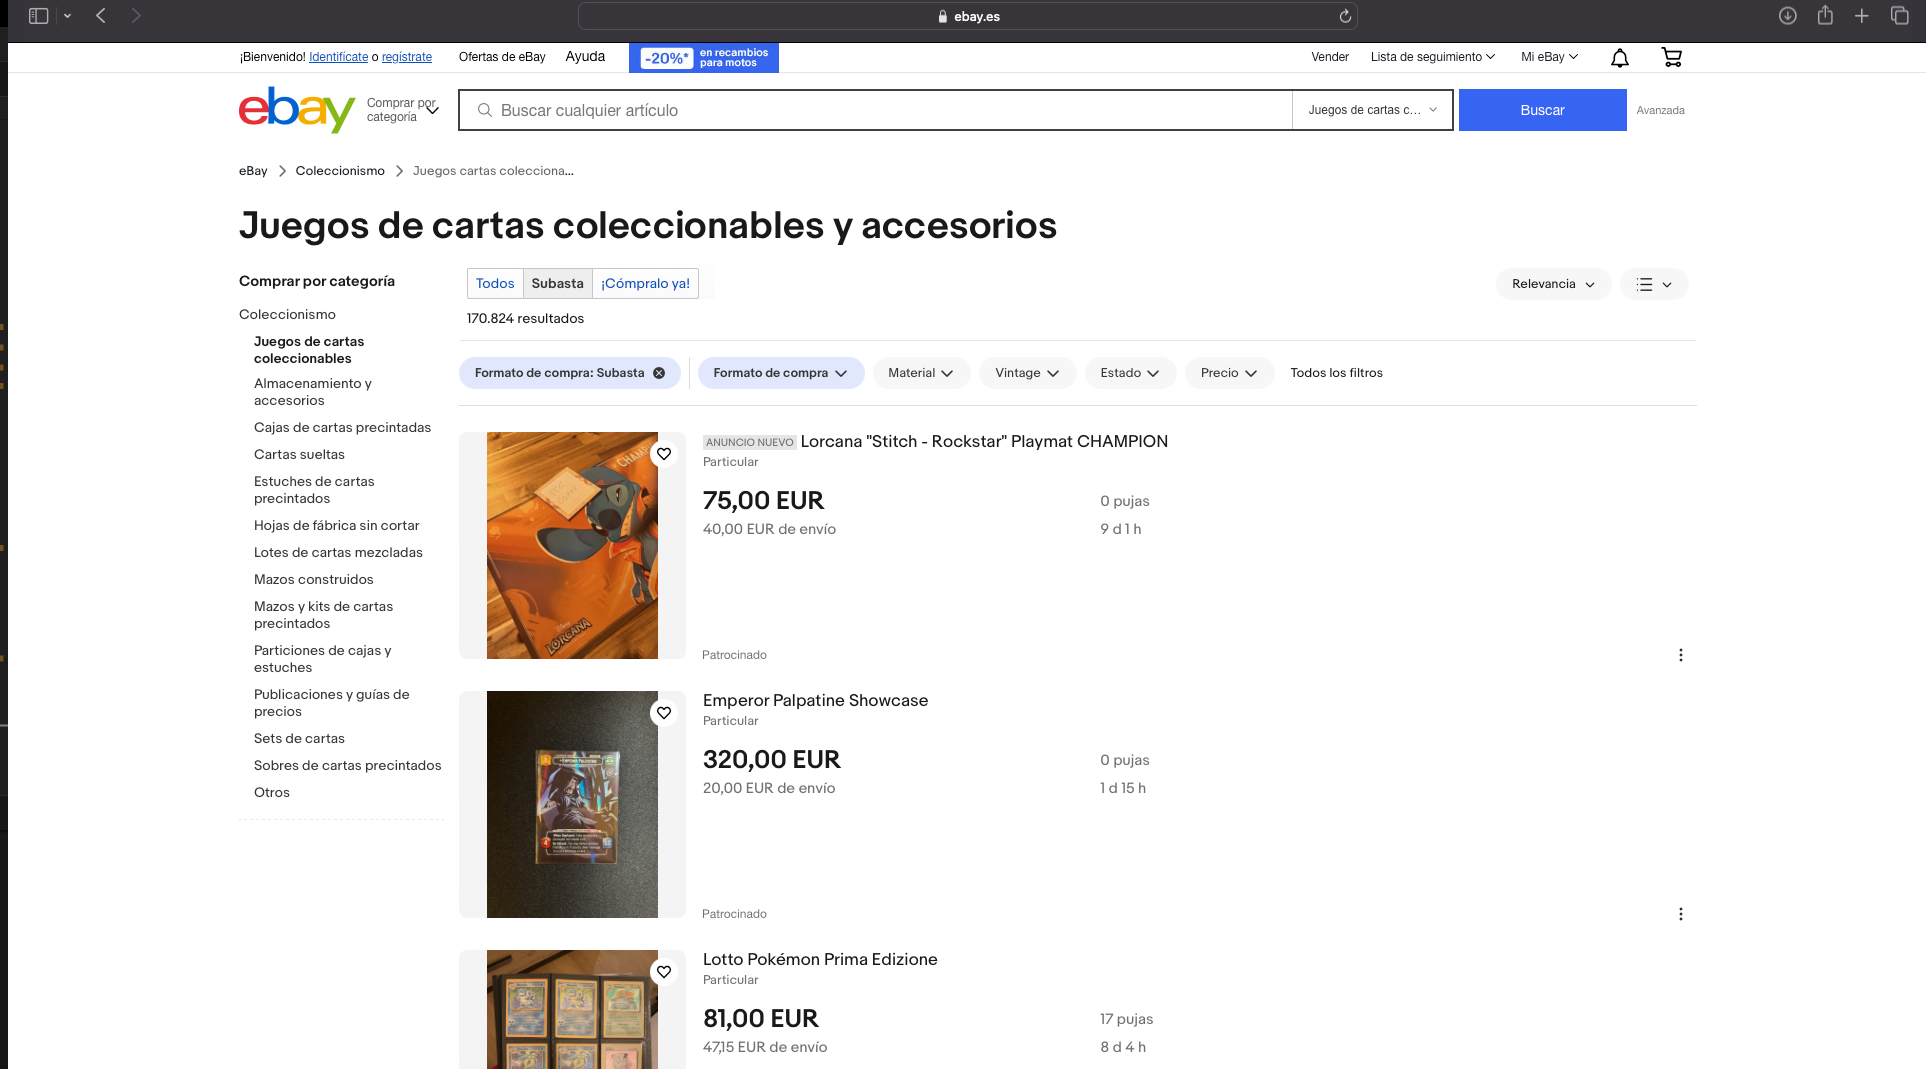
\includegraphics[width=0.9\textwidth]{figures/4-Estudio-viabilidad/4_Ebay.png}
    \caption{Página de subastas de la sección de coleccionismo de cartas de eBay}
    \label{fig:ebay}
    \hypertarget{fig:ebay}{}
\end{figure} 

\subsubsubsection{Ventajas de eBay}
Dentro del marco de LaLiga Fantasy, se destacan las siguientes características:
\begin{itemize}
    \item Para cada producto subastado, la plataforma ofrece la posibilidad de visualizar información detallada que incluye el número de pujas, la cantidad de pujadores, las retractaciones, el tiempo restante en la subasta, y proporciona un historial completo de las pujas realizadas en ese producto. Este historial incluye datos relevantes sobre las pujas, como su valor y la fecha en la que se efectuaron. Además, se brinda acceso a información pertinente sobre los pujadores involucrados.
    \item eBay proporciona a los usuarios la capacidad de configurar pujas automáticas. En este proceso, el comprador define el precio máximo que está dispuesto a pagar por el producto, y la plataforma aumenta automáticamente la oferta en su nombre, siempre que sea necesario, para mantener al comprador como el principal postor hasta alcanzar el límite previamente establecido.
    \item Los usuarios tienen la posibilidad de examinar el perfil del vendedor, explorar otros productos que este tenga en venta y establecer contacto directo con él.
    \item Como vendedor, la plataforma te brinda la capacidad de definir el valor inicial de la puja, decidir si deseas recibir ofertas, establecer la fecha de inicio de la subasta, determinar su duración y habilitar la opción de compra directa a un precio específico de tu elección.
\end{itemize}

\subsubsubsection{Desventajas de eBay}
A continuación, es posible señalar las siguientes desventajas:
\begin{itemize}
    \item La interfaz de usuario muestra una gran cantidad de información, lo que puede resultar confuso para alguien que no está acostumbrado a ella.
    \item Cuando se va a realizar una puja, no aparece una ventana emergente de confirmación de puja o similar por lo que es fácil introducir una puja errónea y, posteriormente, puede resultar complicado retirarla.
    \item Las subastas tienen incrementos de puja predefinidos, lo que significa que no puedes especificar un valor concreto por el que desees pujar.
\end{itemize}

\subsubsubsection{Ventajas del nuevo sistema respecto eBay}
\begin{itemize}
    \item El sistema en desarrollo presentará una interfaz simple e intuitiva, que proporcionará todos los datos esenciales para efectuar una puja con confianza, sin abrumar al usuario con una sobrecarga de información.
    \item El sistema que se desarrollará proporcionará al usuario información sobre las condiciones para retirar una puja antes de su confirmación.
\end{itemize}

% datos de facturación de laliga y juegos fantasy
% https://www.palco23.com/entorno/los-fantasy-se-preparan-para-su-boom-el-negocio-rebasara-416-millones-en-2024
% ebay https://www.ebayinc.com/company/

\section{Valoración de alternativas de solución}

En el presente apartado, se realiza un examen detallado de las diversas alternativas tecnológicas y arquitectónicas disponibles que satisfacen los requisitos previamente establecidos para el proyecto. 

Este análisis implica una evaluación rigurosa de las ventajas y desventajas asociadas a cada opción. La finalidad es identificar la solución más apropiada que no solo cumpla con los requisitos funcionales y no funcionales del proyecto, sino que también se alinee óptimamente con las restricciones y objetivos globales del mismo.

\subsection{Valoración de alternativas para la arquitectura}
A continuación, se presenta una comparación de varias alternativas arquitectónicas para el desarrollo del sistema.
\subsubsection{Arquitectura Monolítica}
La arquitectura monolítica es un enfoque de desarrollo de software en el que una aplicación se construye como una sola unidad. En este caso, todos los componentes del sistema se diseñan y se implementan como un único bloque, que se ejecuta como un único proceso.
Este enfoque en un proyecto pequeño puede ser beneficioso, ya que simplifica el proceso de desarrollo y sobretodo de despliegue. Sin embargo, a medida que el proyecto crece, la arquitectura monolítica se vuelve cada vez más compleja y difícil de mantener. Además, la escalabilidad de la aplicación se ve limitada por la necesidad de escalar el sistema en su conjunto, en lugar de poder escalar componentes individuales de forma independiente.
\begin{figure}[H]
    \centering
    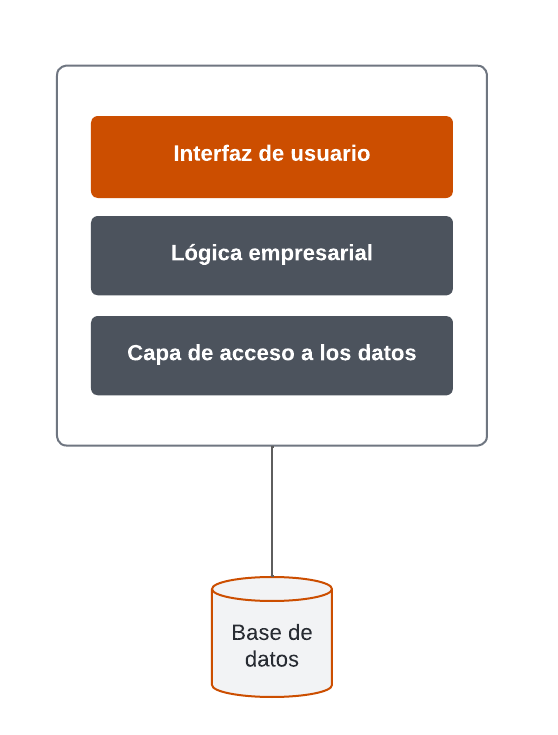
\includegraphics[width=0.4\textwidth]{figures/4-Estudio-viabilidad/4_Monolitica.png}
    \caption{Arquitectura Monolítica}
    \label{fig:arquitectura_monolitica}
    \hypertarget{fig:arquitectura_monolitica}{}
\end{figure}

\subsubsection{Arquitectura de Microservicios}
La arquitectura de microservicios es un enfoque de desarrollo de software en el que una aplicación se construye como un conjunto de servicios pequeños, independientes y altamente escalables. Cada servicio se ejecuta como un proceso separado y se comunica con otros servicios mediante mecanismos ligeros, como una API REST.
Este enfoque permite que los servicios se desarrollen, desplieguen y escalen de forma independiente, lo que facilita la gestión de proyectos complejos. Sin embargo, la arquitectura de microservicios también introduce una mayor complejidad en el desarrollo y la gestión de la aplicación, ya que requiere la implementación de mecanismos de comunicación entre los servicios, así como la gestión de la escalabilidad de cada uno de ellos.
\begin{figure}[H]
    \centering
    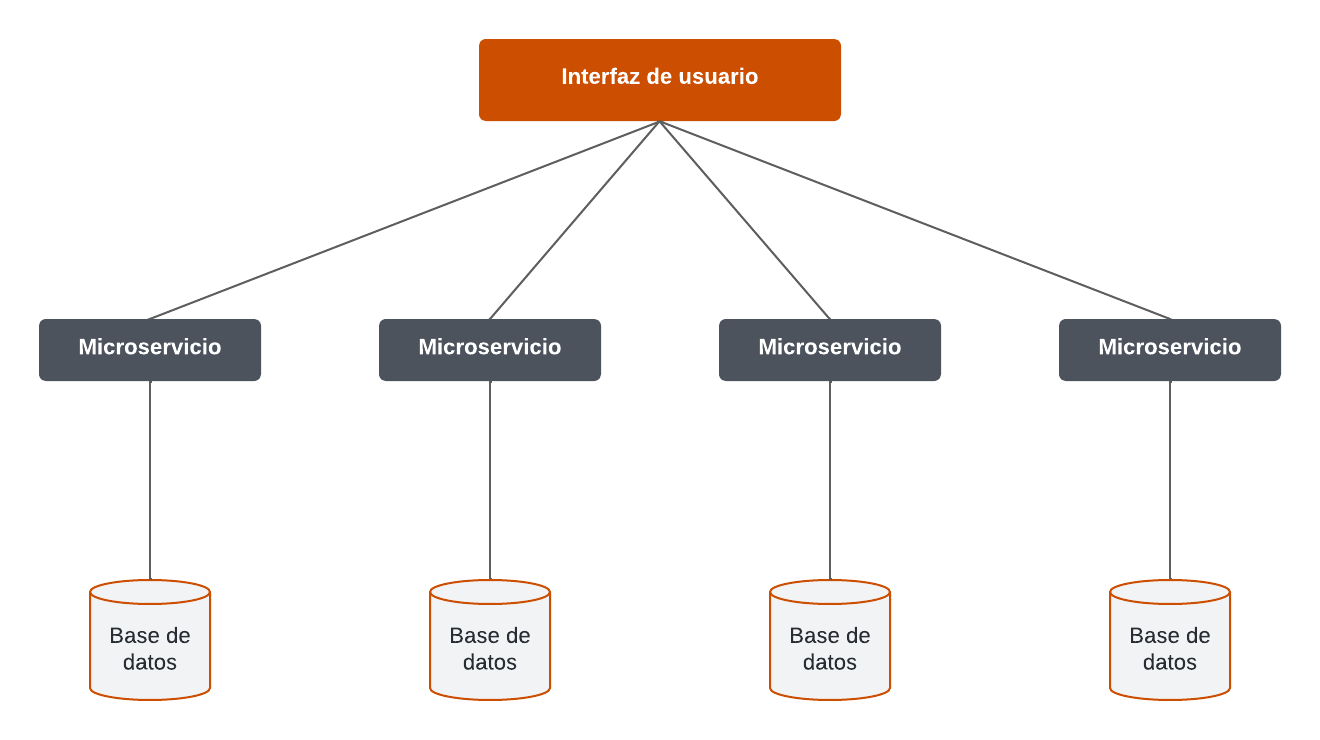
\includegraphics[width=0.7\textwidth]{figures/4-Estudio-viabilidad/4_Microservicios.png}
    \caption{Arquitectura de Microservicios}
    \label{fig:arquitectura_microservicios}
    \hypertarget{fig:arquitectura_microservicios}{}
\end{figure}

\subsubsection{Arquitectura de REST API y WepApp}    
Se caracteriza por una clara división entre cliente y servidor, encapsulados respectivamente en WepApp (frontend) y REST API (backend). Esta separación promueve una organización modular, facilitando el mantenimiento del proyecto al separar de forma clara las distintas responsabilidades. 
Este enfoque es un punto intermedio entre las dos arquitecturas anteriores, ya que permite una mayor flexibilidad en el desarrollo y la gestión de la aplicación, sin introducir una complejidad excesiva. 
\begin{figure}[H]
    \centering
    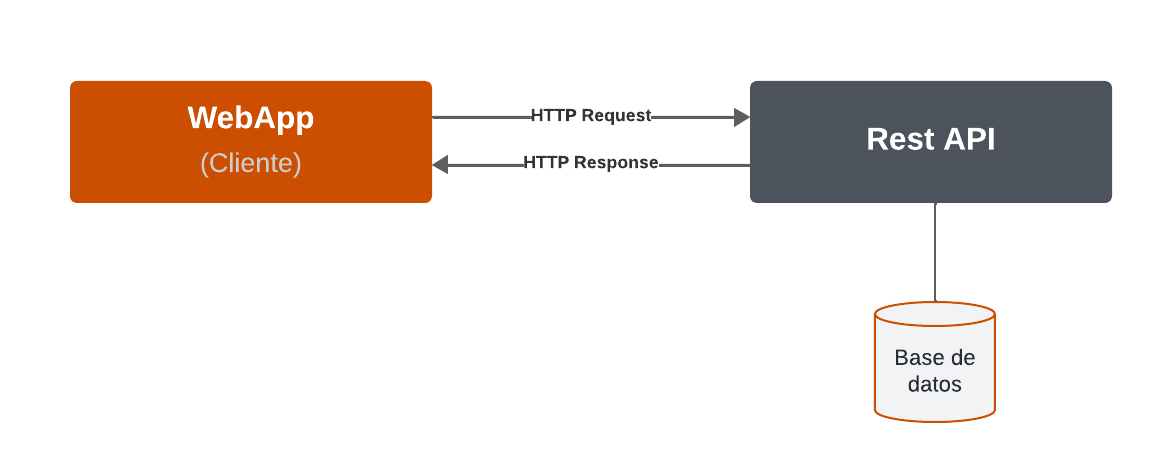
\includegraphics[width=0.7\textwidth]{figures/4-Estudio-viabilidad/4_WebApp_RestApi.png}
    \caption{Arquitectura de REST API y WebApp}
    \label{fig:arquitectura_rest_api_webapp}
    \hypertarget{fig:arquitectura_rest_api_webapp}{}
\end{figure}

\subsubsection{Comparativa de alternativas arquitectónicas}
Mediante la siguiente tabla, se presenta una comparación de las alternativas arquitectónicas previamente mencionadas.

\begin{table}[htb]
    \centering
    \caption{Comparación de Arquitecturas de Software}
    \label{tabla:comparacion_arquitecturas}
    \hypertarget{table:comparacion_arquitecturas}{}
    \begin{tabular}{
       >{\columncolor{rowcolor}\raggedright\arraybackslash}p{4cm}
       >{\raggedright\arraybackslash}p{3cm}
       >{\raggedright\arraybackslash}p{3cm}
       >{\raggedright\arraybackslash}p{3cm} }
    \rowcolor{lightgreen}
    \toprule
    \textbf{Criterio} & \textbf{Arquitectura Monolítica} & \textbf{Arquitectura de Microservicios} & \textbf{API REST y WebApp} \\
    \midrule
    Complejidad Inicial & Baja & Alta & Moderada \\
    \midrule
    Escalabilidad & Limitada & Alta & Moderada \\
    \midrule
    Facilidad de Mantenimiento & Alta en proyectos pequeños & Moderada a baja & Moderada si cada módulo tiene una estructura interna clara \\
    \midrule
    Despliegue & Sencillo & Complejo & Moderado \\
    \midrule
    Gestión de Proyectos & Simple en proyectos pequeños & Requiere coordinación compleja & Balanceada \\
    \midrule
    Independencia de Componentes & No & Sí & Parcial \\
    \midrule
    Adaptabilidad a Cambios & Baja & Alta & Moderada \\
    \midrule
    Recomendado para & Proyectos pequeños y simples & Proyectos grandes y escalables & Proyectos con necesidad de separación clara entre frontend y backend \\
    \bottomrule
    \end{tabular}
\end{table}


\subsubsection{Decisión final de la arquitectura}
Tras un análisis exhaustivo de las alternativas disponibles, se ha optado por implementar una arquitectura de API REST y WebApp.

Esta decisión permite alcanzar un equilibrio entre la simplicidad inherente a la arquitectura monolítica y la escalabilidad ofrecida por la arquitectura de microservicios. Además, esta elección facilita la gestión del proyecto mediante una separación clara entre el frontend y el backend. Tal distinción posibilita el desarrollo y despliegue independiente de cada componente, contribuyendo a la minimización de riesgos asociados a fallos en cadena. 
Además, cada módulo, operando de manera aislada, mejora significativamente la disponibilidad y confiabilidad del sistema.



\subsection{Valoración de alternativas para el Backend}
Es crucial seleccionar una tecnología de backend que no solo soporte eficientemente las operaciones en tiempo real sino que también se integre de manera óptima con el frontend.
A continuación, se presenta un análisis de varias alternativas para el desarrollo del backend teniendo en cuenta estos requisitos.

\subsubsection{Java con Spring Boot}
\coloredUnderline{\href{https://www.java.com/es/}{Java}} es un lenguaje de programación orientado a objetos que destaca por su portabilidad y robustez, siendo ampliamente utilizado en el desarrollo de aplicaciones empresariales. 
La combinación con \coloredUnderline{\href{https://spring.io/projects/spring-boot}{Spring Boot}} permite un desarrollo ágil con una amplia gama de herramientas como Spring Data y Spring Security entre otras. 
Entre sus ventajas, además de las herramientas mencionadas, destacan su escalabilidad, su robustez en el manejo de transacciones y su amplia comunidad. 
Sin embargo, Java con Spring Boot presenta una curva de aprendizaje significativa y, aunque Spring Boot puede manejar aplicaciones en tiempo real mediante Spring WebFlux, su rendimiento en este ámbito puede ser inferior comparado con otras tecnologías. Además, la integración con el frontend, podría no ser la más rápida en términos de desarrollo.

\subsubsubsection{Node.js con Express}
\coloredUnderline{\href{https://nodejs.org/es/}{Node.js}} es un entorno de ejecución para JavaScript en el lado del servidor, conocido por su modelo de I/O no bloqueante y su eficiencia en el manejo de múltiples conexiones simultáneas
La integración de Node.js con \coloredUnderline{\href{https://expressjs.com/es/}{Express}}, un framework ligero y flexible, ofrece una solución óptima para desarrollar aplicaciones web dinámicas.
Esta combinación destaca por su capacidad para gestionar operaciones en tiempo real de manera eficiente y su sinergia natural con tecnologías frontend basadas en JavaScript, facilitando un desarrollo cohesivo y ágil entre el backend y el frontend.
Como desventajas, cabe mencionar que Node.js puede no ser la opción más adecuada para tareas que requieren un alto uso de CPU debido a su naturaleza de ejecución de un solo hilo, ya que su rendimiento en este ámbito puede ser inferior al de otras tecnologías.

\subsubsection{Python con Django}
\coloredUnderline{\href{https://www.python.org/}{Python}}, un lenguaje de programación de alto nivel, se caracteriza por su versatilidad y amplia gama de bibliotecas. Utilizado ampliamente en 
aplicaciones empresariales combinado con \coloredUnderline{\href{https://www.djangoproject.com/}{Django}}, un framework de alto nivel que se enfoca en el desarrollo rápido y eficiente.
Como ventajas, destacan su desarrollo rápido, sus excelentes capacidades de seguridad y su buena documentación.
Aunque Django puede ser configurado para soportar aplicaciones en tiempo real mediante Django Channels, su rendimiento en estos escenarios puede no ser tan óptimo como el de Node.js. Además, aunque Django asegura una buena integración con el frontend, puede no ser la opción más ágil para aplicaciones que requieren una interacción constante.



\subsubsection{Comparativa de alternativas para el Backend}
En la siguiente tabla, se presenta una comparación de las alternativas para el desarrollo del Backend.
\begin{table}[H]
    \centering
    \begin{tabular}{ 
       >{\columncolor{rowcolor}\raggedright\arraybackslash}p{3cm} 
       >{\raggedright\arraybackslash}p{3cm} 
       >{\raggedright\arraybackslash}p{3cm} 
       >{\raggedright\arraybackslash}p{3cm} }
        \rowcolor{lightgreen}
    \toprule
    \textbf{Criterio} & \textbf{Java con Spring Boot} & \textbf{Node.js con Express} & \textbf{Python con Django} \\
    \midrule
    \textbf{Modelo de Programación} & Orientado a objetos, con énfasis en inyección de dependencias. & Basado en eventos y callbacks. & Orientado a componentes/modelos con énfasis en la reutilización de código. \\
    \midrule
    \textbf{Funcionalidad en tiempo real} & Buen manejo de transacciones pero menos óptimo para tiempo real. & Excelente para operaciones en tiempo real gracias a su eficiencia en I/O. & Posible pero requiere más configuración para tiempo real. \\
    \midrule
    \textbf{Integración con Frontend} & Buena, puede requerir esfuerzos adicionales. & Natural y fluida. & Buena, pero puede necesitar configuraciones extra. \\
    \midrule
    \textbf{Escalabilidad} & Alta, pero con escalabilidad vertical. & Alta, con facilidad para escalar horizontalmente. & Moderada, con algunas limitaciones en escalabilidad. \\
    \midrule
    \textbf{Seguridad} & Fuertes capacidades de seguridad. & Requiere implementaciones adicionales para seguridad. & Seguridad integrada y robusta. \\
    \bottomrule
    \end{tabular}
    \caption{Comparación de Tecnologías para el Backend}
    \label{tabla:comparacion_backend}
    \hypertarget{table:comparacion_backend}{}
    \end{table}

    
\subsubsection{Decisión final del Backend}
Considerando las necesidades del sistema a desarrollar, para soportar subastas en tiempo real y una integración fluida con el frontend la opción más adecuada es Node.js con Express.


\subsection{Valoración de alternativas para el Frontend}
A continuación, se presenta un análisis de alternativas para el desarrollo del frontend.

\subsubsection{React}
\coloredUnderline{\href{https://es.react.dev}{React}} es una biblioteca de JavaScript desarrollada y mantenida por Facebook, centrada en la construcción de interfaces de usuario a través de componentes reutilizables. Se caracteriza por su virtual DOM y su enfoque declarativo.

Entre sus ventajas, destacan su amplia comunidad, su rendimiento optimizado con Virtual DOM y su flexibilidad en la elección de estilos y componentes. 
Como desventajas cabe mencionar las actualizaciones frecuentes que implican mantenerse al día con los cambios y que necesita integración con otras herramientas para ser una solución completa.


\subsubsection{Angular}
\coloredUnderline{\href{https://angular.io/}{Angular}} es un framework de desarrollo web mantenido por Google, conocido por su enfoque en aplicaciones de página única (SPA). Utiliza TypeScript como lenguaje principal y proporciona un entorno robusto y completo para el desarrollo.

Entre sus ventajas, destaca su ecosistema completo, promueve un estilo de desarrollo coherente y mantenible y, además, cuenta con una comunidad activa y un amplio soporte de Google, lo que garantiza actualizaciones y soporte continuo.
Sin embargo, Angular puede ser excesivo para proyectos pequeños, ya que su curva de aprendizaje es pronunciada y su configuración inicial puede ser compleja.

\subsubsection{Vue.js}
\coloredUnderline{\href{https://vuejs.org/}{Vue.js}} es un framework progresivo para la construcción de interfaces de usuario, creado por Evan You. Se destaca por su facilidad de adopción, su sistema reactividad y su enfoque en la simplicidad.

Entre sus ventajas, destacan su sintaxis sencilla, su buena documentación y su facilidad de integración en proyectos existentes.
Aunque su uso va en aumento, su comunidad es más pequeña en comparación con React o Angular, lo que se traduce en menos librerías y recursos disponibles.

\subsubsection{Comparativa de alternativas para el Frontend}
A continuación, se presenta una comparación de las alternativas para el desarrollo del Frontend.

\begin{table}[H]
    \centering
    \begin{tabular}{ 
       >{\columncolor{rowcolor}\raggedright\arraybackslash}p{2.5cm} 
       >{\raggedright\arraybackslash}p{3.5cm} 
       >{\raggedright\arraybackslash}p{3.5cm} 
       >{\raggedright\arraybackslash}p{3.5cm} }
        \rowcolor{lightgreen}
    \toprule
    
    \textbf{Criterio} & \textbf{React} & \textbf{Angular} & \textbf{Vue.js} \\
    \midrule
    \textbf{Velocidad y Rendimiento} & Alto con Virtual DOM. Optimizado para cambios dinámicos de UI. & Buen rendimiento, pero puede ser más lento en proyectos grandes debido a su complejidad. & Rendimiento similar a React, con optimizaciones en la actualización de la UI. \\
    \midrule
    \textbf{Mantener el Estado} & Requiere bibliotecas adicionales como Redux para manejo complejo del estado. & Gestión de estado integrada, adecuada para aplicaciones complejas. & Sistema reactividad sencillo, para manejo de estado complejo requiere la biblioteca Vuex. \\
    \midrule
    \textbf{Comunidad} & Muy grande y activa, con un ecosistema extenso. & Amplia y soportada por Google, con muchas empresas adoptándolo. & Creciente y entusiasta, con un enfoque en la facilidad de uso. \\
    \midrule
    \textbf{Curva de Aprendizaje} & Moderada; JSX y el ecosistema pueden requerir tiempo de aprendizaje. & Elevada; TypeScript y su arquitectura completa requieren más tiempo para aprender. & Baja; Vue es considerado fácil de aprender, especialmente para principiantes. \\
    \midrule
    \textbf{Escalabilidad} & Muy escalable con un enfoque modular y reutilizable. & Diseñado para aplicaciones empresariales escalables y complejas. & Escalable, pero más adecuado para proyectos de tamaño mediano. \\
    \midrule
    \textbf{Ecosistemas y Módulos} & Rico ecosistema con una gran cantidad de módulos y herramientas. & Ecosistema completo con soluciones integradas para muchas necesidades. & Ecosistema más pequeño aunque en crecimiento, con módulos y librerías en aumento. \\
    \bottomrule
    \end{tabular}
    \caption{Análisis Comparativo de Frameworks y Bibliotecas de Frontend}
    \label{tabla:comparacion_frontend}
    \hypertarget{table:comparacion_frontend}{}
\end{table}

\subsubsection{Decisión final del Frontend}
Tras una evaluación detallada de las distintas opciones disponibles y en función de los requisitos específicos del sistema a desarrollar, se ha determinado que React es la tecnología más adecuada para el frontend.

Esta decisión se basa, principalmente, en la gran comunidad de React y en la rica colección de recursos disponles.

\subsection{Valoración de alternativas para la Base de Datos}
Por último, se presenta un análisis de alternativas para la base de datos del sistema.

\subsubsection{MySQL}
\coloredUnderline{\href{https://www.mysql.com/}{MySQL}} es un sistema de gestión de bases de datos relacional de código abierto, ampliamente utilizado en aplicaciones web. 

Entre sus ventajas, destacan su amplia adopción lo que conlleva una gran cantidad de recursos y documentación disponibles, su fiabilidad y robustez y su facilidad de uso. 

Por otro lado, MySQL puede no ser la opción más adecuada para aplicaciones que requieren de operaciones avanzadas de análisis y procesamiento de datos, ya que su rendimiento en este ámbito puede ser inferior al de otras bases de datos.

\subsubsection{MongoDB}
\coloredUnderline{\href{https://www.mongodb.com/}{MongoDB}} es una base de datos NoSQL orientada a documentos, diseñada para la escalabilidad y la flexibilidad. Se caracteriza por su capacidad para manejar grandes volúmenes de datos y su esquema flexible.

Entre sus ventajas, destacan su flexibilidad, permite que la base de datos crezca con la aplicación añadiendo nuevos campos a los documentos.
Además, MongoDB es altamente escalable y puede manejar grandes volúmenes de datos de manera eficiente.

Sin embargo, MongoDB puede no ser la opción más adecuada para aplicaciones que requieren transacciones ACID complejas, ya que su modelo de consistencia eventual puede no ser adecuado para todas las aplicaciones.

\subsubsection{PostgreSQL}
\coloredUnderline{\href{https://www.postgresql.org/}{PostgreSQL}} es un sistema de gestión de bases de datos relacional de código abierto y gratuito, conocido por su robustez, escalabilidad y soporte para transacciones ACID.

Entre sus ventajas, destacan su cumplimiento con los estándares SQL, su soporte para transacciones ACID y su capacidad para manejar grandes volúmenes de datos asegurando la integridad y seguridad de los mismos.

Como inconvenientes, cabe mencionar que PostgreSQL puede ser más lento que otras bases de datos en operaciones de lectura y escritura para bases de datos pequeñas ya que está enfocada en manejar un gran volumen de datos,
 y su curva de aprendizaje puede ser pronunciada para usuarios no familiarizados con SQL.

\subsubsection{Comparativa de alternativas para la Base de Datos}
En la siguiente tabla, se presenta una comparación de las alternativas para la base de datos del sistema.
\begin{table}[H]
    \centering
    \begin{tabular}{ 
       >{\columncolor{rowcolor}\raggedright\arraybackslash}p{3cm} 
       >{\raggedright\arraybackslash}p{3cm} 
       >{\raggedright\arraybackslash}p{3cm} 
       >{\raggedright\arraybackslash}p{3cm} }
        \rowcolor{lightgreen}
    \toprule
    \textbf{Criterio} & \textbf{MySQL} & \textbf{MongoDB} & \textbf{PostgreSQL} \\
    \midrule
    \textbf{Tipo de Base de Datos} & Relacional & NoSQL & Relacional \\
    \midrule
    \textbf{Modelo de Datos} & Tablas y Filas & Documentos JSON/BSON & Tablas y Filas \\
    \midrule
    \textbf{Lenguaje de Consulta} & SQL & MongoDB Query Language (MQL) & SQL \\
    \midrule
    \textbf{Escalabilidad} & Escalabilidad vertical y soporte para horizontal & Escalabilidad horizontal mediante sharding & Escalabilidad vertical y horizontal \\
    \midrule
    \textbf{Transacciones} & Soporte completo de ACID & Soporte parcial de ACID en ciertas operaciones & Soporte completo de ACID \\
    \midrule
    \textbf{JSON} & Soporte limitado mediante campos JSON & JSON nativo & Soporte avanzado de JSON y JSONB \\
    \midrule
    \textbf{Flexibilidad de Esquema} & Esquemas rígidos & Esquemas flexibles& Esquemas rígidos \\
    \midrule
    \textbf{Rendimiento} & Alto rendimiento en lecturas & Alto rendimiento en escrituras & Alto rendimiento en lecturas y escrituras \\
    \bottomrule
    \end{tabular}
    \caption{Comparativa entre MySQL, MongoDB y PostgreSQL}
    \label{tabla:comparacion_bases_datos}
    \hypertarget{table:comparacion_bases_datos}{}
\end{table}


\subsubsection{Decisión final de la Base de Datos}
Tras un análisis detallado de las distintas opciones disponibles y en función de los requisitos específicos del sistema a desarrollar, se ha determinado que MongoDB es la tecnología más adecuada para la base de datos. 

Esta elección se basa en un \textit{trade-off}, es decir, se acepta la falta de integridad referencial y la consistencia eventual a cambio de una mayor flexibilidad y escalabilidad en el manejo de datos que es lo que se necesita para el sistema a desarrollar.


\subsection{Selección final de alternativas de solución}

Se han seleccionado las siguientes tecnologías como alternativas de solución: Node.js con Express para el backend, React.js para el frontend, y MongoDB como base 
de datos. 

Estas decisiones conforman una arquitectura \textbf{MERN} (MongoDB, Express, React, Node.js), ejemplificada en la \coloredUnderline{\hyperlink{fig:arquitectura_mern}{Figura \ref*{fig:arquitectura_mern}: \nameref*{fig:arquitectura_mern}}}. 

Esta arquitectura presenta diversas ventajas, tales como la familiaridad de los desarrolladores con las tecnologías involucradas, el amplio soporte y documentación disponibles debido a su uso común en el desarrollo de aplicaciones web actuales,
y la facilidad de integración entre las tecnologías.

Se puede consultar más información sobre la arquitectura MERN en el siguiente enlace: \coloredUnderline{\href{https://www.mongodb.com/resources/languages/mern-stack}{MERN Stack}}.

\begin{figure}[H]
    \centering
    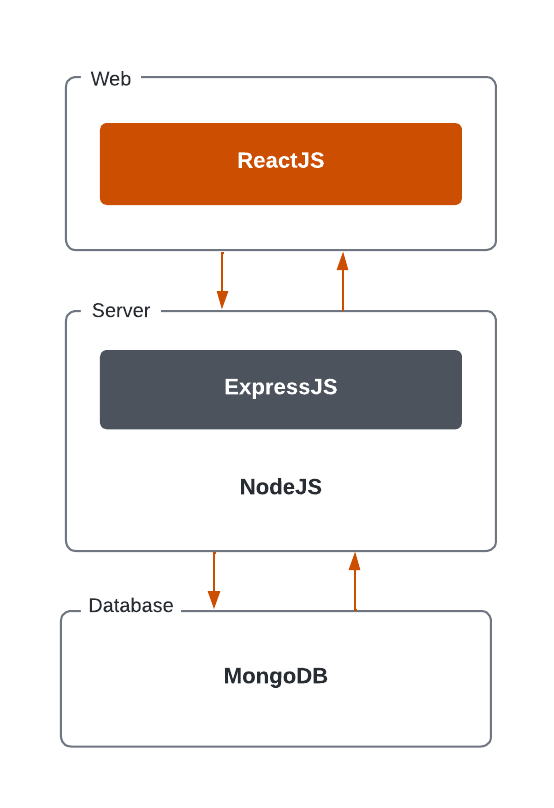
\includegraphics[width=0.4\textwidth]{figures/4-Estudio-viabilidad/4_MERN2.png}
    \caption{MERN Stack: MongoDB, Express, React, Node.js}
    \label{fig:arquitectura_mern}
    \hypertarget{fig:arquitectura_mern}{}
\end{figure}



\newpage
\chapter{PLANIFICACIÓN Y GESTIÓN DEL TFG}
\newpage

\newpage
\section{PLANIFICACIÓN DEL PROYECTO}

\subsection{Identificación de Interesados}


\subsection{OBS y PBS}


\subsection{Planificación Inicial. WBS}


\subsection{Riesgos}

\subsubsection{Plan de Gestión de Riesgos} 

\subsubsection{Identificación de Riesgos}

\subsubsection{Registro de Riesgos} 



\subsection{Presupuesto Inicial}

\subsubsection{Presupuesto de Costes}

\subsubsection{Presupuesto de Cliente} 


\newpage
\section{EJECUCIÓN DEL PROYECTO}

\subsection{Plan Seguimiento de Planificación}

\subsection{Bitácora de Incidencias del Proyecto}

\subsection{Riesgos}


\newpage
\section{CIERRE DEL PROYECTO}

\subsection{Planificación Final}

\subsection{Informe Final de Riesgos}

\subsection{Presupuesto Final de Costes}

\subsection{Informe de Lecciones Aprendidas}



\newpage
\chapter{ANÁLISIS DEL SISTEMA DE INFORMACIÓN}

\newpage


\section{DEFINICIÓN DEL SISTEMA}

\subsection{Determinación del Alcance del Sistema}


\newpage
\section{ESTABLECIMIENTO DE REQUISITOS}

\subsection{Obtención de los Requisitos del Sistema} 

\subsection{Identificación de Actores del Sistema} 

\subsection{Especificación de Casos de Uso}

\textcolor[rgb]{0.65,0.16,0}{Ejemplo de tabla para especificación de casos de uso}

\begin{table}[htbp]
  \centering
  \caption{Especificación Caso de Uso 1}
    \begin{tabular}{p{20.855em}r}
\cmidrule{1-1}    \rowcolor[rgb]{ .949,  .949,  .949} \multicolumn{1}{p{20.855em}}{\textbf{Nombre del caso de uso}} & \multicolumn{1}{r}{\cellcolor[rgb]{ 1,  1,  1}} \\
\cmidrule{1-1}    \multicolumn{1}{p{20.855em}}{Registro} & \multicolumn{1}{r}{} \\
    \midrule
    \rowcolor[rgb]{ .949,  .949,  .949} \multicolumn{2}{p{31.64em}}{\textbf{Descripción}} \\
    \midrule
    \multicolumn{2}{p{31.64em}}{Un usuario no registrado debe poder registrarse en el sistema mediante su cuenta de Google, lo que hará que automáticamente se inicie sesión en la aplicación.} \\
    \bottomrule
    \end{tabular}%
  \label{espec_caso_uso_1}%
  \vspace{-4mm}
\end{table}%

\newpage
\section{IDENTIFICACIÓN DE SUBSISTEMAS DE ANÁLISIS}

\subsection{Descripción de los Subsistemas} 

\subsection{Descripción de los Interfaces entre Subsistemas}


\newpage
\section{ANÁLISIS DE LOSac CASOS DE USO}

\subsection{Caso de Uso 1} 

\textcolor[rgb]{0.65,0.16,0}{Ejemplo de tabla para análisis de casos de usos}

\begin{table}[H]
  \centering
  \vspace{-5mm}
  \caption{Análisis del Caso de Uso 1}
    \begin{tabular}{p{7.5em}p{24.145em}}
    \toprule
    \rowcolor[rgb]{ .871,  .918,  .965} \multicolumn{2}{p{31.645em}}{\textbf{Registro}} \\
    \midrule
    \rowcolor[rgb]{ .906,  .902,  .902} \textbf{Precondiciones} & \cellcolor[rgb]{ 1,  1,  1}El usuario no debe haber iniciado sesión nunca. \\
    \midrule
    \rowcolor[rgb]{ .906,  .902,  .902} \textbf{Postcondiciones} & \cellcolor[rgb]{ 1,  1,  1}- \\
    \midrule
    \rowcolor[rgb]{ .906,  .902,  .902} \textbf{Actores} & \cellcolor[rgb]{ 1,  1,  1}Usuario no registrado \\
    \midrule
    \rowcolor[rgb]{ .906,  .902,  .902} \textbf{Descripción} & \cellcolor[rgb]{ 1,  1,  1}El usuario accederá a la pantalla principal de la aplicación cuando no se está registrado, y seleccionará el botón de inicio de sesión, que, al ser la primera vez, registrará.Seleccionará la cuenta de Google con la que desee registrarse y el sistema completará el resto del registro. \\
    \midrule
    \rowcolor[rgb]{ .906,  .902,  .902} \textbf{Escenarios          Secundarios} & \cellcolor[rgb]{ 1,  1,  1} El usuario no tiene cuenta de Google: escenario que puede ser posible si accede a la aplicación a través del App Market. En este caso se le solicitará crear una cuenta. \\
    \bottomrule
    \end{tabular}%
\end{table}%
 
\subsection{Caso de Uso 2}


\newpage
\section{ANÁLISIS DE CLASES}

\subsection{Diagrama de Clases} 

\subsection{Descripción de las Clases}


\newpage
\section{DEFINICIÓN DE INTERFACES DE USUARIO}

\subsection{Descripción de la Interfaz} 

\subsection{Definición del aspecto de la interfaz}

\subsection{Descripción del Comportamiento de la Interfaz} 

\subsection{Diagrama de Navegabilidad}


\newpage
\section{ESPECIFICACIÓN DEL PLAN DE PRUEBAS}


\newpage
\chapter{DISEÑO DEL SISTEMA DE INFORMACIÓN}
	

\newpage


\section{DISEÑO DE CASOS DE USO REALES}

\subsection{Caso de Uso 1.1} 

\subsubsection{Diagramas de Interacción (Comunicación y Secuencia)} 

\subsubsection{Diagramas de Estados de las Clases} 
 
\subsubsection{Diagramas de Actividades} 


\subsection{Caso de Uso 1.2}


\newpage
\section{DISEÑO DE CLASES}

\subsection{Diagrama de Clases}


\newpage
\section{DISEÑO DE LA ARQUITECTURA DE MÓDULOS DEL SISTEMA}

\subsection{Diseño de Módulos del Sistema}

\subsection{Diseño de Comunicaciones entre Módulos}

\subsection{Revisión de la Interfaz de Usuario}


\newpage
\section{DISEÑO FÍSICO DE DATOS}

\subsection{Descripción del SGBD Usado} 

\subsection{Integración del SGBD en Nuestro Sistema} 

\subsection{Diagrama E--R} 


\newpage
\section{DISEÑO DE LA MIGRACIÓN Y CARGA INICIAL DE DATOS}


\newpage
\section{ESPECIFICACIÓN TÉCNICA DEL PLAN DE PRUEBAS}

\subsection{Pruebas Unitarias} 

\subsection{Pruebas de Integración y del Sistema} 

\subsection{Pruebas de Usabilidad y Accesibilidad} 

\subsubsection{Diseño de Cuestionarios} 

\subsubsection{Actividades de las Pruebas de Usabilidad} 


\subsection{Pruebas de Accesibilidad} 

\subsection{Pruebas de Rendimiento} 


\newpage
\chapter{CONSTRUCCIÓN DEL SISTEMA DE INFORMACIÓN}


\newpage


\section{PREPARACIÓN DEL ENTORNO DE GENERACIÓN Y CONSTRUCCIÓN}

\subsection{Estándares y normas seguidos}


\subsection{Lenguajes de programación}


\subsection{Herramientas y programas usados para el desarrollo}


\newpage
\section{GENERACIÓN DEL CÓDIGO DE LOS COMPONENTES Y PROCEDIMIENTOS}

\textcolor[rgb]{0.65,0.16,0}{Ejemplos de tablas descripción de clases}

\begin{table}[H]
\vspace{-4mm}
  \centering
  \caption{Descripción de diseño de LoginScreen}
    \begin{tabular}{p{8.645em}rr}
    \toprule
    \rowcolor[rgb]{ .851,  .886,  .953} \multicolumn{3}{p{31.285em}}{\textbf{LoginScreen}} \\
    \midrule
    \rowcolor[rgb]{ .949,  .949,  .949} \multicolumn{3}{p{31.285em}}{\textbf{Descripción}} \\
    \midrule
    \multicolumn{3}{p{31.285em}}{Es la encargada de las acciones y la renderización de la pantalla de inicio de sesión.} \\
    \midrule
    \rowcolor[rgb]{ .906,  .902,  .902} \multicolumn{3}{p{31.285em}}{\textbf{Atributos propuestos}} \\
    \midrule
    \multicolumn{3}{p{31.285em}}{-} \\
    \midrule
    \rowcolor[rgb]{ .906,  .902,  .902} \multicolumn{3}{p{31.285em}}{\textbf{Métodos propuestos}} \\
    \midrule
    \textbf{signInWithGoogle} & \multicolumn{2}{p{22.64em}}{Hace una llamada al objeto Fire para el inicio de sesión con Firebase authentication mediante una cuenta de Google.} \\
    \midrule
    \textbf{render} & \multicolumn{2}{r}{} \\
    \bottomrule
    \end{tabular}%
\end{table}%


\begin{table}[htbp]
  \centering
  \caption{Descripción de diseño de HomeScreen}
    \begin{tabular}{p{10em}rr}
    \toprule
    \rowcolor[rgb]{ .851,  .886,  .953} \multicolumn{3}{p{31.285em}}{\textbf{HomeScreen}} \\
    \midrule
    \rowcolor[rgb]{ .949,  .949,  .949} \multicolumn{3}{p{31.285em}}{\textbf{Descripción}} \\
    \midrule
    \multicolumn{3}{p{31.285em}}{Es la encargada de las acciones y la renderización de la pantalla de emergencia.} \\
    \midrule
    \rowcolor[rgb]{ .906,  .902,  .902} \multicolumn{3}{p{31.285em}}{\textbf{Atributos propuestos}} \\
    \midrule
    \multicolumn{3}{p{31.285em}}{-} \\
    \midrule
    \rowcolor[rgb]{ .906,  .902,  .902} \multicolumn{3}{p{31.285em}}{\textbf{Métodos propuestos}} \\
    \midrule
    \textbf{componentWillMount} & \multicolumn{2}{r}{} \\
    \midrule
    \textbf{emergencyCalling} & \multicolumn{2}{p{21.285em}}{Es el método encargado de redirigir la aplicación hacia el marcador con el 112 marcado.} \\
    \midrule
    \textbf{warnProtectors} & \multicolumn{2}{p{21.285em}}{[Falta implementar] Es el encargado de generar un mensaje de aviso a los protectores creando notificaciones push.} \\
    \midrule
    \textbf{render} & \multicolumn{2}{r}{} \\
    \bottomrule
    \end{tabular}%
\end{table}%

\newpage
\section{EJECUCIÓN DE LAS PRUEBAS UNITARIAS}


\newpage
\section{EJECUCIÓN DE LAS PRUEBAS DE INTEGRACIÓN}


\newpage
\section{EJECUCIÓN DE LAS PRUEBAS DEL SISTEMA}

\subsection{Prueba de Usabilidad}

\subsection{Pruebas de Accesibilidad} 
 
\subsubsection{Revisión Preliminar} 

\subsubsection{Evaluación de Conformidad} 

\subsubsection{Checklist del WCAG 2.1} 

\subsubsection{Accesibilidad con Dispositivos Móviles} 


\newpage
\section{ELABORACIÓN DE LOS MANUALES DE USUARIO}

\subsection{Manual de Instalación} 

\subsection{Manual de Ejecución} 

\subsection{Manual de Usuario} 

\subsection{Manual del Programador}


\newpage
\section{CONSTRUCCIÓN DE LOS COMPONENTES Y PROCEDIMIENTOS DE MIGRACIÓN Y CARGA INICIAL DE DATOS}



\newpage
\chapter{IMPLANTACIÓN Y ACEPTACIÓN DEL SISTEMA}
	

\newpage

\section{ESTABLECIMIENTO DEL PLAN DE IMPLANTACIÓN}


\newpage
\section{CARGA DE DATOS AL ENTORNO DE OPERACIÓN}


\newpage
\section{PRUEBAS DE IMPLANTACIÓN DEL SISTEMA}


\newpage
\section{PREPARACIÓN DEL MANTENIMIENTO DEL SISTEMA}


\newpage
\section{ESTABLECIMIENTO DEL ACUERDO DE NIVEL DE SERVICIO}


\newpage
\section{PRESENTACIÓN Y APROBACIÓN DEL SISTEMA Y PASO A PRODUCCIÓN}


\newpage
\chapter{CONCLUSIONES Y AMPLIACIONES}
\newpage

\section{CONCLUSIONES}

\newpage
\section{AMPLIACIONES} 


\newpage
\chapter*{ANEXOS}
\addcontentsline{toc}{chapter}{ANEXOS}
\newpage
\phantomsection
\section*{PLAN DE GESTIÓN DE RIESGOS}
\addcontentsline{toc}{section}{PLAN DE GESTIÓN DE RIESGOS}

\newpage
\section*{CONTENIDO ENTREGADO EN LOS ANEXOS} 
\addcontentsline{toc}{section}{CONTENIDO ENTREGADO EN LOS ANEXOS}

\subsection*{Contenidos} 

\textcolor[rgb]{0.65,0.16,0}{Ejemplo de como especificar los contenidos entregados}

Además de este documento, se hace entrega de una carpeta comprimida ``.zip'' en la que ahora se describirán sus contenidos. Se estructurará también la organización del código fuente.

\begin{itemize}
	\item \textbf{Planificación\_TFG.mpp} -> Archivo de Microsoft Project que contiene la planificación del proyecto entera.
	\item \textbf{Presupuesto-GuardMe\_TFG.xlsx} -> Archivo Microsoft Excel que contiene los cálculos del presupuesto del proyecto.
	\item \textbf{Diagramas} -> Carpeta que contiene todos los diagramas utilizados en este documento.
	\begin{itemize}
		\item \textit{Diagrama\_de\_paquetes.png}
		\item \textit{Diagrama\_firestore.png}
		\item \textit{Diagrama\_navegabilidad.png}
		\item \textit{Diagrama\_secuencia\_enviar.png}
		\item \textit{Diagrama\_secuencia\_visualizar.png}
		\item \textit{Diagrama\_UML-Diseño.png}
		\item \textit{Diagrama\_UML-Analisis.png}
	\end{itemize}
	\item \textbf{TFG\_codigo.zip} -> Carpeta comprimida con todo el código fuente.
\end{itemize}

Ahora se mostrará el contenido de dicha carpeta comprimida que contiene todo el código fuente de la aplicación la cual esta dividida a su vez en dos carpetas:

\paragraph*{AuthServerGuardMe}
Contiene el código que se aloja en \textit{Heroku} para darle funcionalidad al servidor. La clase principal es la llamada \texttt{mainAuthServer.js}.

\paragraph*{GuardMe}
Contiene el código fuente de la aplicación y se compone de las siguientes carpetas:
\begin{itemize}
	\item \textbf{assets} -> Carpeta que contiene los elementos gráficos usados en la aplicación. Se subdivide en una carpeta llamada \textit{images} que contiene todas las imagenes utilizadas para la construcción de la aplicación.
	\item \textbf{components} -> Carpeta que contiene el código para todos los componentes creados.
	\item \textbf{constants} -> Carpeta que contiene el código
	\item \textbf{docs} -> Carpeta que contiene los archivos html generados por JSDoc.
	\item \textbf{files} -> Carpeta en la que se encuentras los futuros archivos de Términos y Condiciones y Política de Privacidad entre otros.
	\item \textbf{modules\_LICENSES} -> Carpeta que contiene una por una todas las licencias de las librerías utilizadas en el desarrollo.
	\item \textbf{navigation} -> Carpeta que contiene las clases relativas a la navegación de la aplicación.
	\item \textbf{objects} -> Carpeta que contiene los objetos utilizados en el desarrollo que en este caso ha sido solo Fire.js.
	\item \textbf{screens} -> Carpeta que contiene todas las pantallas, agrupadas a su vez en subcarpetas que identifican la pantalla sobre la que están relacionadas.
	\item \textbf{styles} -> Carpeta que contiene todos los estilos de las pantallas, agrupadas a su vez en subcarpetas que siguen la misma estructura que \textit{screens}.
	\item \textbf{App.js} -> Clase principal y encargada de que comience la aplicación entera.
	\item \textbf{LICENSE} -> Licencia sobre el código fuente.
	\item \textbf{README.md} -> Archivo con la descripción del proyecto para la documentación y el repositorio de GitHub.
	\item \textbf{package.json} -> Archivo que contiene las librerías utilizadas en el proyecto.
	\item \textbf{app.json} -> Archivo que contiene la configuración de la aplicación.
	\item \textbf{configJSDoc.json} -> Archivo de configuración para la creación de documentación por parte de JSDoc.
	\item \textbf{Otros archivos} -> Los demás archivos no son relevantes ya que muchos se generan por defecto y los demás son configuraciones propias de expo.
\end{itemize}

\newpage
\nocite{*} %El comando bibliography enseña solo las referencias que se hayan usado en el texto. Este comando permite "no citar" todas y así que aparezcan.
\bibliographystyle{ieeetr} 
\bibliography{references}

\newpage





\end{document}
